To structure the design process, an iterative process is used to come up with a design. First a shape is needed, from the design sensitivity 



For the new shape, the trajectory is determined using a fixed \gls{sym:alpha}. The aerocapture phase is then tuned to a 


\begin{figure}[h!]
		\vspace{-1cm}
		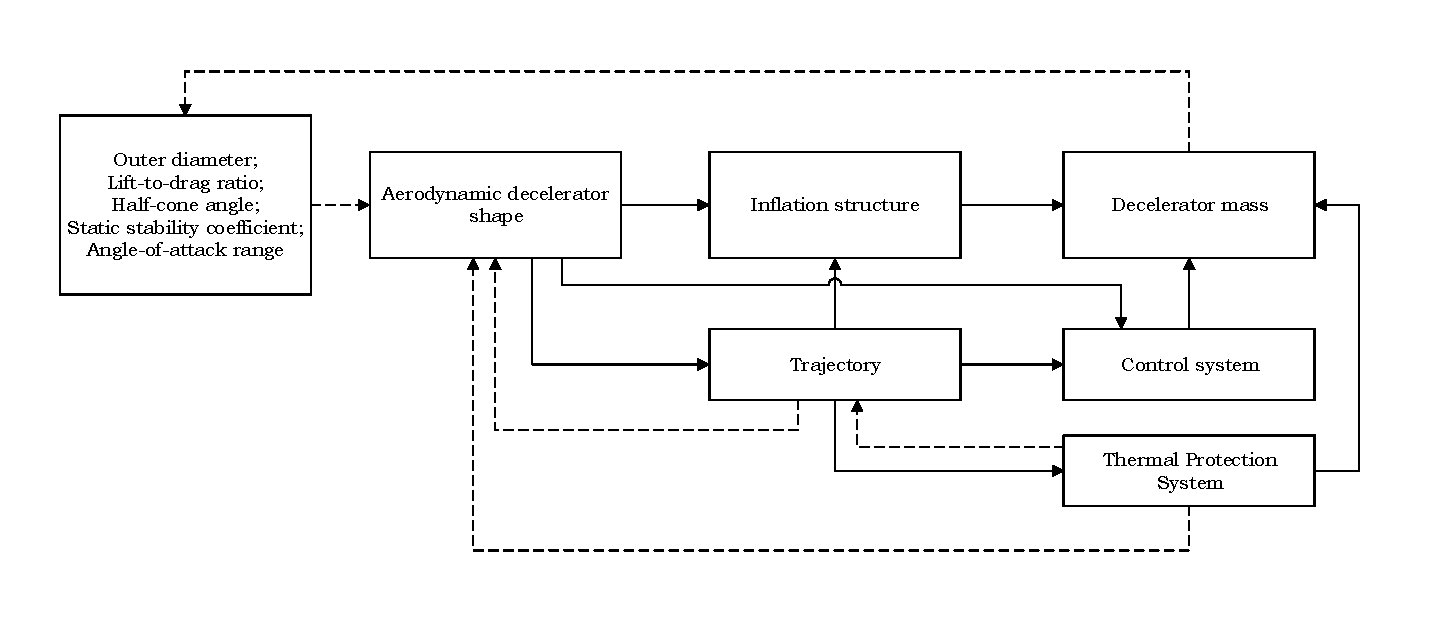
\includegraphics[width=0.96\textwidth]{./Figure/DesignIterationPhilosophy.pdf}
		\vspace{-2.3cm}
		\caption{The iterative design process flowchart}
		\label{fig:rot}
\end{figure}